
\section{Project Tango}

Project Tango ist eine Technologie Plattform für Android Tablets und Smartphones von Google’s Advanced Technology and Projects Group (ATAP). Das Ziel dieser Plattform ist es Motion Tracking (Positionierung), Depth Perception (Tiefeninformation/Pointcloud) und Area Learning (Lokalisierung) auf mobile Endgeräte zu bringen, um verschiedenste Anwendungs-Szenarien abzudecken. Typische Szenarien sind Indoor Navigation, Virtual Reality Anwendungen, Vermessungs- und Rekonstruktions Software und Augmented Reality Anwendungen.\\

Es ermöglicht in erster Linie ein Tracking von Positionsänderungen des Geräts im Raum und bietet somit eine genaue relative Lokalisierung. Mit Hilfe dieser Lokalisierung und der Hinzunahme von visuellen Merkmalen im Raum, ist das Gerät in der Lage, seine Umgebung kennenzulernen und gegebenenfalls die Lokalisierung zu korrigieren oder aber in einer bereits erlernten Umgebung zu ermitteln. Zusätzlich bietet Project Tango die Möglichkeit mit Hilfe eines Tiefensensors eine Pointcloud der Tiefeninformation pro Bildausschnitt zu liefern, um Anwendungen auch Räumliche Informationen bereitzustellen.  \citep{Proje19:online} \\

\subsection{Geräte und Hardware}

Da das Project Tango zum Zeitpunkt der Verfassung dieser Thesis noch unter Entwicklung steht, gibt es von Google die Entwickler Prototypen. Das Erste Gerät im Smartphone Format, welches in Abbildung \ref{fig:tango-device} rechts unten zu erkennen ist, wurde bereits durch eine neue Generation rechts oben ersetzt. Dieses 7\dq Tablet verfügt, wie in Abbildung \ref{fig:tango-device} links zu erkennen, über einen Infrarot Laser Projektor, eine Fisheye Camera und eine normale 4 Megapixel Kamera auf der Rückseite. Zudem sind, wie von aktuellen Smartphones bekannt, ein Beschleunigungssensor, Umgebungslichtsensor, Barometer, Kompass, GPS und ein Gyroskop verbaut. Das Gerät wird von einem NVIDIA Tegra K1 Prozessor betrieben und verfügt über 4GB Arbeitsspeicher. \citep{Proje19:online} Mit diesem Gerät wurden die später beschriebenen Techniken umgesetzt und evaluiert.  \\

\begin{figure}[h]
  \centering
	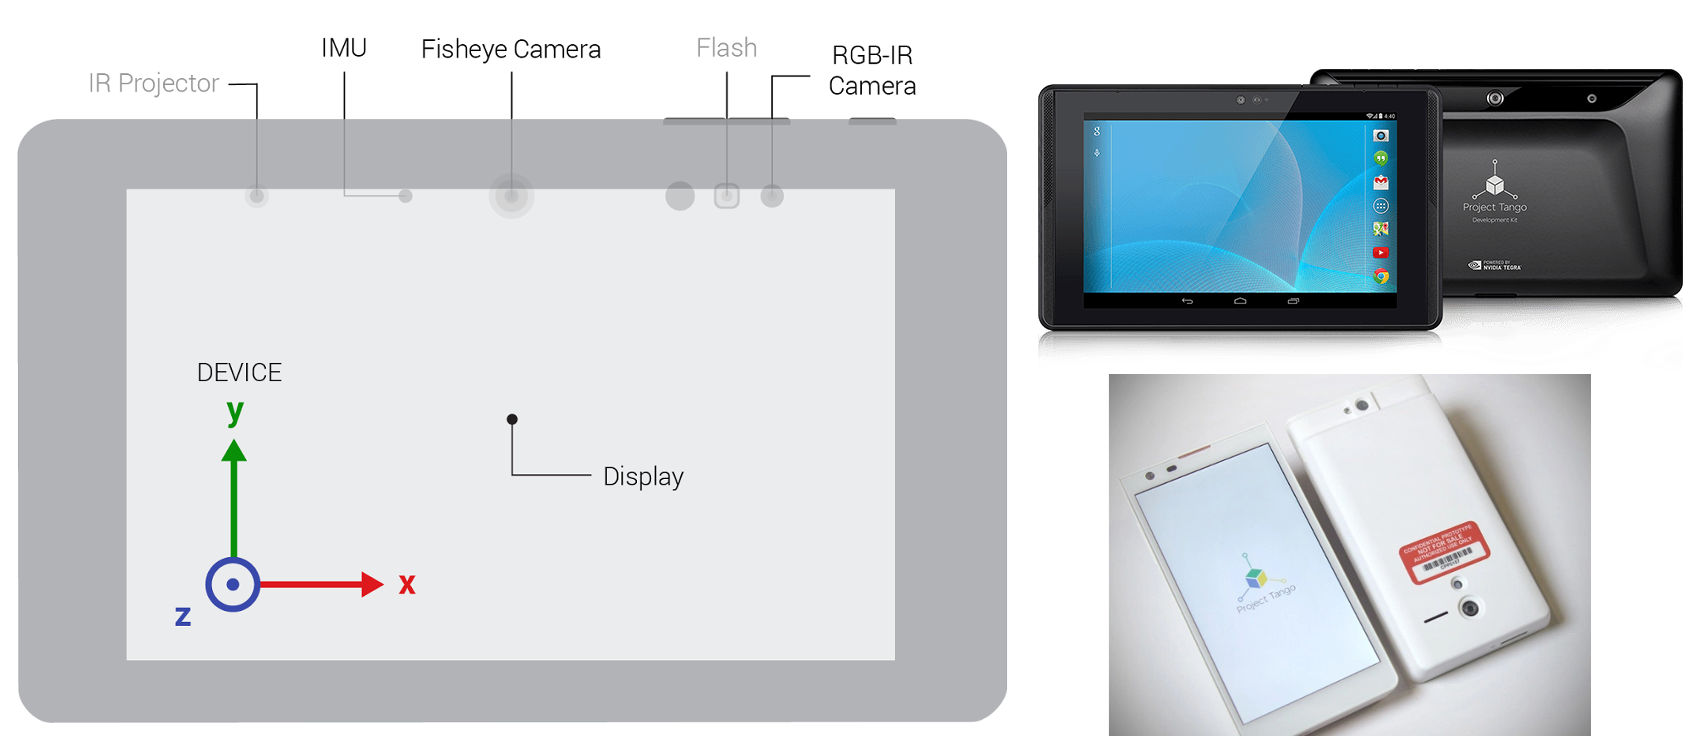
\includegraphics[width=1.0\textwidth]{content/images/theory/tango-device.png} 
  \caption{Links: schematischer Aufbau der Google Project Tango Hardware. Rechts: Das aktuelle Entwickler Gerät im Tablet Faktor (oben) und das alte Entwickler Gerät im Smartphone Faktor (unten). Übernommen von \citet{GoogleDevelopers:online}}
  \label{fig:tango-device}
\end{figure}

\subsection{Konzepte und Schnittstellen}

Generell betrachtet ist das Project Tango eine Plattform, die Computer Vision nutzt, um dem Gerät die Möglichkeit bietet seine relative Positionierung in der umgebenen Szene live zu bestimmen. Auf den Geräten kommt Googles Android zum Einsatz, weshalb zu beachten ist, dass es sich bei der Platform nur Bedingt um eine Echtzeit Umgebung handelt. Das liegt daran, dass der Linux Kernel keine Garantien für die zeitlich präzise Ausführung von Instruktionen  auf Grund von Scheduling geben kann. Google weist daher darauf hin, dass das System als \enquote{soft-realtime} betrachtet werden sollte. Daher sollten Messergebnisse verschiedener Sensoren unter Berücksichtigung ihrer Aufnahme Zeitstempel verwendet werden. \citep{GoogleDevelopersConcepts:online} \\

\subsubsection{Motion Tracking}

Um die relative Bewegung vom Start des Project Tango Systems bestimmen zu können nutzt es \enquote{visual-inertial odometry}. \citep{GoogleDevelopersConcepts:online}
Dabei handelt es sich um eine erweiterte Variante von Visual Odometry. 
Das von \citet{nister2004visual} veröffentlichte Verfahren Visual Odometry ist in der Lage aus einfachen Video Inhalten in Echtzeit die Bewegung der Kamera zu bestimmen. 
Hierzu werden zunächst übergreifende Features, zum Beispiel Punkte aus der \citet{harris1988combined} Kantenerkennung, über mehrere Bilder des Videos bestimmt, woraus mit Hilfe des 5-point Algorthmus und durch Answendung von RANSAC eine bestmögliche Approximation der Kamera Transformation bestimmt wird. \citep{nister2004visual} \\

Project Tango lässt an dieser Stelle die internen Sensoren zur Rotation, Orientierung und Bewegung mit in die Bestimmung der Kamera Transformation einfließen um so ein akurateres Ergebnis erziehlen zu können. Über eine längere Messzeit oder eine größere Entfernung vom Ursprung kann es jedoch zu kleinen Abweichungen kommen. Außerdem existiert zum aktullen Zeitpunkt noch ein \enquote{drift} Problem, was zu großen Messfehlern führen kann. Es wird jedoch versucht diese Probleme mit dem Konzept \enquote{Area Learning}, beschrieben in Kapitel \ref{subsec:area-learning}, zu lösen. \citep{GoogleDevelopersConcepts:online}
Wie genau das Verfahren aussieht, welche Techniken zur Feature Detection oder Feature Matching genutzt wird und welche Features hierfür erkannt werden ist nicht bekannt.  \\

\subsubsection{Deph Perception}

Zur Tiefenmessung ist die Project Tango Hardware mit einem kalibrierten Infrarot Laser Projektor ausgestattet. Dieser streut Infrarot Punkte mit einer Auflösung von 320 x 180 Punkten in den Raum, um dann, mit Hilfe von Aufnahmen der RGB Kamera, eine Punktewolke der Tiefeninformation zu bestimmen. Auf Grund einer ausgewogenen Konfiguration zwischen Messbereich, Messfehlern und dem Energieverbrauch, liegt der Messbereich der Sensorkombination, laut \citet{GoogleDevelopersConcepts:online}, zwischen einem halben und vier Metern. \\

Dadurch dass diese Technologie auf der Aufnahme von projiziertem Infrarot Licht basiert, ist ein Einsatz der Tiefenmessung außerhalb geschlossener Räume nicht möglich. \citep{GoogleDevelopersConcepts:online} Außerdem entstehen Messfehler durch reflektierende,  lichtabsorbierende oder zu komplex strukturierte Oberflächen, wie zum Beispiel Metalle, LCD Monitore oder Hochflor Teppiche. \\

Die zuvor erwähnten Punktewolken werden in dem eigens definierten XYZij Format von der Entwicklungsschnittstelle zurück gegeben. Dabei handelt es sich pro Punkt um die \(X\),\(Y\) und \(Z\) Koordinaten sowie der Spalte \(i \) und der Zeile \(j\). \citep{GoogleDevelopersConcepts:online} Man spricht dabei von einer organisierten Punktewolke, da durch die \(i\) und \(j\) Koordinaten die direkten Nachbarn, ausgehend von dem Aufnahmeblickwinkel, eines Punktes bestimmt werden können. Hieraus ist es möglich, die sogenannten \enquote{depth-maps} zu bestimmen, für die es viele verschiedene Computer Vision Verfahren zur Bestimmung von Objekten, Strukturen und Fluchtpunkten gibt !!! !!! . Die Ermittlung der Spalten \(i\) und Zeilen \(j\) sind jedoch laut \citet{GoogleDevelopersKnownIssues:online} noch nicht in den Schnittstellen enthalten.\\ 

\citet{GoogleDevelopersConcepts:online} weist darauf hin, dass das Generieren von Polygon basierten Rekonstruktionen noch nicht in den Schnittstellen enthalten sind. Es gibt jedoch freie Drittbibliotheken, wie das Robot Operating System \citep{ROS} oder die Point Cloud Library \citep{pcl}. Die für eine weitere Verarbeitung genutzt werden können.

\subsubsection{Area Learning} \label{subsec:area-learning}

Area Learning bezeichnet den Prozess indem Project Tango Geräte in der Lage sind durch visuelle Hinweise die umgebenen Welt kennenzulernen und auf die Position des Gerätes zu schließen. 
Es ermöglicht somit eine Unterstützung für Motion Tracking und löst das Problem das Gerät in einer bereits bekannten Umgebung zu lokalisieren, wie in Abbildung \ref{fig:area-learning} links zu erkennen.
Project Tango bietet außerdem die Möglichkeit diese visuellen Hinweise und Ihre Position im Raum in sogenannten \enquote{Area Description Files} zu speichern und wiederzuverwenden. \citep{GoogleDevelopersConcepts:online}\\

Wie bereits erwähnt entstehen bei Motion Tracking Messfehler über eine längere Strecke. 
Während diese Strecke mit einem Project Tango Gerät abgelaufen wird, ermittelt es fortlaufend die Position und den Pfad, den der Nutzer im Raum gegangen ist. 
Erkennt es währnend der Strecke visuelle Merkmale vom Area Learning, wird der Pfad anhand der Positionen der Merkmale ensprechend angepasst. 
Project Tango unterscheidet hier zwischen zwei Manipulationen, \enquote{loop closures}, zur Zusammenführung des Pfads wenn ein Kreis gelaufen wurde, und \enquote{drift corrections}, um den erwähnten drift Effekt bei zu wenigen optischen Features im visual-inertial odometry. 
Die dirft correction ist in Abbildung \ref{fig:area-learning} rechts zu erkennen.
\citep{GoogleDevelopersConcepts:online}\\

\begin{figure}[h]
  \centering
	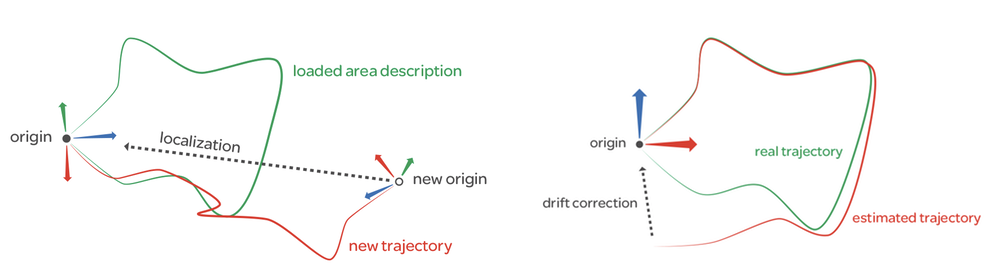
\includegraphics[width=1.0\textwidth]{content/images/theory/tango-area-learning.png} 
  \caption{Links: Lokalisierungsprozess durch Area Learning. Rechts: Korrigierung von Motion Tracking anhand gelernter Merkmale . Übernommen von \citet{GoogleDevelopers:online}}
  \label{fig:area-learning}
\end{figure}

Figure 1: Correcting the Estimated Trajectory
Without drift correction, a game or application using a virtual 3D space aligned with the real world may encounter inaccuracies in motion tracking after extended use. For example, if a door in a game world corresponds with a door frame in the real world, after accumulating drift, the game door may appear in the middle of the real world wall instead of in the door frame.

Localization using area descriptions

In addition to drift correction, a device with a loaded area description knows where it is within the learned area relative to where the original learning started. This process is called localization. Without localizing to an area description, a device's starting point is lost every time you end the session. This ability to learn an area and localize against that area is required if you want to create a consistent experience within the same mapped space, such as having virtual objects appear in the same location as the last time the user visited an area.

Figure 2 shows what happens when a device starts from a new origin and moves back into an area it has learned before.


Figure 2: Localizing to a Saved Area Description
Project Tango devices depend on the visual diversity of the area to localize. If you are in an area with many identical rooms or in a completely empty room with blank walls, it will be difficult to localize.

Creating and saving an Area Description

There are two ways to create an Area Description File. The simplest is to use an application like Project Tango Explorer to create the ADF, and have your application load it. The second is to use the Project Tango APIs to handle the learning, saving, and loading all within your application. Depending on your settings, you can learn a new area or append to an existing ADF.

A room may look quite different when standing in different positions, if furniture is moved around, or during the day than it does at night. If current conditions are similar to when you create the area description, localization is more likely to succeed. If localization is not occuring, the area descriptions may be too different from the current conditions.

Because there are many reasons why an area may change in appearance, you might create multiple area description files for a single physical location under different conditions and select the correct one that will be most similar to the conditions the user will have during their session. Alternatively, you could append multiple area learning sessions onto the same ADF to capture visual descriptions of the environment from every position and angle, under every variation of lighting or environmental change within one file.

Our UX Best Practices has additional tips on creating ADFs and using area learning.

Possible use cases

As mentioned, learning and loading area descriptions has many advantages. You can now intentionally align the device's coordinate frame with a pre-existing coordinate frame so that content in a game or app always appears in the same physical location.

Another advantage is for multi-player experiences, where two users can localize to the same coordinate frame, shared through a cloud service. This allows multiple people to interact in the same physical space where all of their relative positions are known. Although the Project Tango APIs do not natively support data sharing in the cloud, it is possible to use Google Cloud Storage and the Google Play Games API to implement this.

Some use cases may include a space owner making available an area description of their environment, such as a retail store or public space. These area descriptions may have been created by an expert user, such as a store manager. This would allow end users to localize precisely within that physical space, for example with location-aware shopping experience.

Important: Saved area descriptions do not directly record images or video of the location, but rather contain descriptions of images of the environment in a very compressed form. While those descriptions can’t be directly viewed as images, it is in principle possible to write an algorithm that can reconstruct a viewable image. Therefore, you must ask the user for permission before saving any of their learned areas to the cloud or sharing areas between users to protect the user's privacy, just as you would treat images and video.
Area learning and using area descriptions are powerful features and we’re excited to see what developers come up with for offering new user experiences.

Using Learning Mode and loaded Area Description Files

Depending on your settings for learning mode or whether you loaded an ADF, the behavior of some aspects of the Project Tango APIs will vary.

In this table, the left two columns denote whether you have learning mode on, and whether you have loaded a previously-stored area description. Depending on the status of those two things, you may or may not be able to save an area description. For example, if you don't have learning mode on, you cannot save an area description file. If you have learning mode on, and have loaded an area description file, you can only save again once you have localized against the loaded ADF.

Also, if you aren't in learning mode, and don't have an ADF loaded, you cannot get pose data using the TANGO_COORDINATE_FRAME_AREA_DESCRIPTION frame of reference. If you have an ADF loaded, you can get pose data from that frame of reference once your device localizes to the loaded ADF.

\subsection{Einordnung zu Augmented Reality}

Um das Project Tango in den zuvor erwähnten technologischen Charakteristika einordnen zu können, wird zunächst einmal auf die technischen Details der Plattform eingegangen. \\
